% it/figures/data_pipeline/fig_manifold.tex — versione italiana
\begin{figure}[!ht]
    \centering
    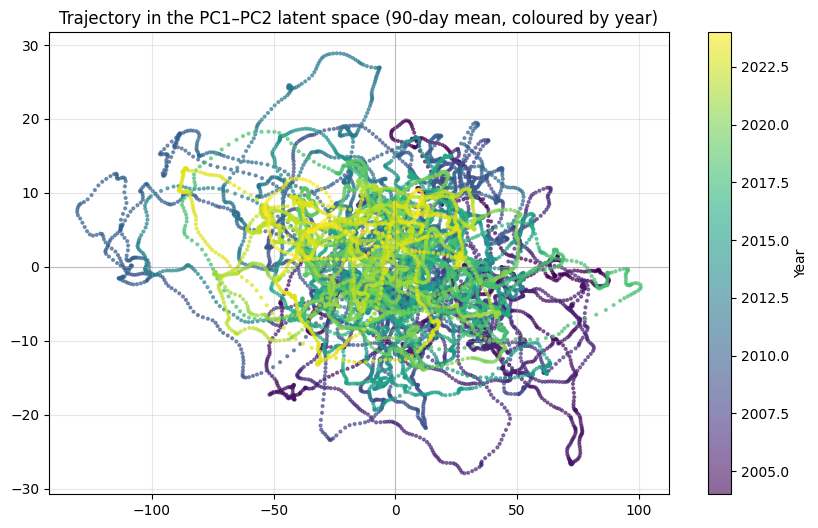
\includegraphics[width=0.85\textwidth]{figures/data_pipeline/fig_manifold.png}
    \caption[La varietà latente piatta dei profili AMOC.]{\textbf{La varietà dei
    profili verticali dell'AMOC è piatta.} Ogni punto è un profilo, collocato dalle
    sue due coordinate latenti --- PC1 (intensità) e PC2 (ridistribuzione verticale).
    Un autoencoder non lineare addestrato sugli stessi profili non li ricostruisce
    meglio della PCA lineare a nessuna dimensione latente (scarto da $-0.06$ a $-0.15$
    punti percentuali; vedi Tabella~\ref{tab:ae-gap}), confermando che due coordinate
    rettilinee catturano la struttura senza distorsione.}
    \label{fig:manifold}
\end{figure}
